\chapter{Probabilistic Planning with Sequential Monte Carlo Methods}
\label{chapter:smcp}
\section*{Article details}


Thomas, V.*, Piché, A.*, , Ibrahim, C., Bengio, Y. and Pal, C. ``Probabilistic Planning with Sequential Monte Carlo methods''. In \emph{International Conference on Learning Representations (ICLR) 2019}.

This work was done jointly with Alexandre Pich\'{e} during the summer 2018 at Mila and ElementAI and was presented at ICLR 2019. 
\section*{Foreword}
The original intuition for this work  was that it should be possible to have a tree search planning algorithm where interesting (\emph{i.e} might get high return) branches were reinforced and less interesting branches cut off. Using control as inference was a natural way to associate the return a branch might get to the probability it would have to be reinforced or cut.

To the best of our knowledge, there is only one article that framed planning as an inference problem~\citep{attias2003planning} and it was in a very specific setting with strong assumptions.
We realized that our idea was intimately linked with sequential Monte Carlo methods and that our algorithm could be framed as an instance of a particle filter.
In control theory, there is a duality between estimating the current state and controlling the dynamics to the desired goal. While particle filters are typically used for estimation, here, within the context of control as inference, we are able to design a particle filter algorithm for control.


\section*{Impact since publication}
This paper already has some citations and follow-up works using our formulation of planning as inference and our algorithm~\citep{wang2019dual, lioutas2022critic}. An evalution paper, \citep{byravan22eval}, found that SMCP performed favorably compared to CEM, both on performance and computational complexity
        ``[...] on the \textbf{harder GTTP tasks SMC slightly outperforms CEM}. We use SMC throughout the paper as it makes better use of the proposal [distribution] compared to CEM 
        [...]
        \textbf{CEM uses a significantly larger computational budget than our SMC planner} which is non-iterative; in spite of this SMC is still quite competitive with CEM across all tasks [...]''

A book~\citep{belousov2021reinforcement} cites SMCP as a promising direction for planning: ''Recent research in probabilistic dynamic models and planning
with sequential Monte Carlo methods viewing control as an inference problem demonstrate the advantages of probabilistic plan
ning in MPC and may be \textbf{one of the most promising directions}[to improve MPC in a black box environment].''


\section*{Personal contribution}
\begin{itemize}
    \item Major contribution on the theoretical understanding of the method.
        Making the link with the two-filter formula~\citep{bresler1986two} and smoothing/forward-backward algorithms
    \item Determining the expression for the update (maximum entropy advantage)
        and writing the proofs in the appendix
    \item Designing and performing the toy experiment~\Cref{fig:toy_sis} and \Cref{fig:toy_sir}
    \item Creating \Cref{fig:graphical_model}, \Cref{fig:tree} and \Cref{fig:alphabeta}
    \item Writing of the paper alongside with Alexandre
\end{itemize}

\newpage
\begin{abstract}
In this work, we propose a novel formulation of planning which views it as a probabilistic inference problem over future optimal trajectories. This enables us to use sampling methods, and thus, tackle planning in continuous %
domains using a fixed computational budget.  We design a new algorithm, Sequential Monte Carlo Planning, by leveraging classical methods in Sequential Monte Carlo and Bayesian smoothing in the context of \textit{control as inference}.  %
Furthermore, we show that Sequential Monte Carlo Planning can capture multimodal policies and can quickly learn continuous control tasks. %
\end{abstract}

\section{Introduction}

To exhibit intelligent behaviour machine learning agents must be able to learn quickly, predict the consequences of their actions, and explain how they will react in a given situation. These abilities are best achieved when the agent efficiently uses a model of the world to plan future actions. To date, planning algorithms have yielded very impressive results. For instance, Alpha Go~\citep{silver2017mastering} relied on Monte Carlo Tree Search (MCTS)~\citep{kearns2002sparse} to achieve super human performances. Cross entropy methods (CEM) \citep{rubinstein2004unified} have enabled robots to perform complex nonprehensile manipulations \citep{finn2017deep} and algorithms to play successfully Tetris \citep{szita2006learning}. In addition, iterative linear quadratic regulator (iLQR) \citep{kalman1960contributions, kalman1964linear, todorov2005generalized} enabled humanoid robots tasks to get up from an arbitrary seated pose \citep{tassa2012synthesis}. 


Despite these successes, these algorithms make strong underlying assumptions about the environment.
First, MCTS requires a discrete setting, limiting most of its successes to discrete games with known dynamics.
Second, CEM assumes the distribution over future trajectories to be Gaussian, i.e. unimodal. Third, iLQR assumes that the dynamics are locally linear-Gaussian, which is a strong assumption on the dynamics and would also assume the distribution over future optimal trajectories to be Gaussian. For these reasons, planning remains an open problem in environments with continuous actions and complex dynamics. In this paper, we address the limitations of the aforementioned planning algorithms by creating a more general view of planning that can leverage advances in deep learning (DL) and probabilistic inference methods. This allows us to approximate arbitrary complicated distributions over trajectories with non-linear dynamics.


We frame planning as density estimation problem over optimal future trajectories in the context of \textit{control as inference} \citep{dayan1997using, toussaint2006probabilistic, toussaint2009robot, rawlik2010approximate, rawlik2012stochastic, ziebart2010modeling, levine2013variational}.  This perspective allows us to make use of tools from the inference research community and, as previously mentioned, model any distribution over future trajectories. The planning distribution is complex since trajectories consist of an intertwined sequence of states and actions. Sequential Monte Carlo (SMC) \citep{stewart1992use, gordon1993novel, kitagawa1996monte} methods are flexible and efficient to model such a distribution by sequentially drawing from a simpler proposal distribution.
From the SMC perspective, the policy can be seen as the proposal and a learned model of the world as the propagation distribution. This provides a natural way to combine model-free and model-based RL.


\textbf{Contribution.} We depict the problem of planning as one of density estimation that can be estimated using SMC methods. We introduce a novel planning strategy based on the SMC class of algorithms, in which we treat the policy as the proposed distribution to be learned. We investigate how our method empirically compares with existing model-based methods and a strong model-free baseline on the standard benchmark Mujoco~\citep{todorov2012mujoco}. 


\section{Background}
\subsection{Control as inference}
\label{sec:control_as_inference}

We consider the general case of a Markov Decision Process (MDP) $\{\gS, \gA, \penv, r, \gamma, \mu\}$ where $\gS$ and $\gA$ represent the state and action spaces respectively. We use the letters $s$ and $a$ to denote states and actions, which we consider to be continuous vectors. Further notations include: $\penv(s' |s, a)$ as the state transition probability of the environment, $r(s, a)$ %
as the reward function, and $\gamma \in [0, 1)$ as the discount factor. $\mu$ denotes the probability distribution over initial states.

This work focuses on an episodic formulation, with a fixed end-time of $T$. We define a trajectory as a sequence of state-action pairs $\traj_{t:T}=\{(s_t,a_t), \ldots,(s_T, a_T) \}$, and we use the notation $\pi$ for a policy which represents a distribution over actions conditioned on a state. Here $\pi$ is parametrized by a neural network with parameters $\parampol$. The notation %
$q_\parampol(\traj_{1:T}) = \mu(s_1) \prod_{t \geq 1}^{T-1} \penv(s_{t+1}|s_t, a_t) \prod_{t \geq 1}^{T} \pi_\parampol(a_t|s_t)$
denotes the probability of a trajectory $\traj_{1:T}$ under policy $\pi_\parampol$. 


\setlength{\wrapoverhang}{\marginparwidth}
\addtolength{\wrapoverhang}{\marginparsep}
\begin{wrapfigure}{r}[-1mm]{.5\linewidth}%
\centering
\resizebox{.95\linewidth}{!}{
\begin{tikzpicture}
\tikzstyle{main}=[circle, minimum size = 5mm, thick, draw =black!80, node distance = 7mm]
\tikzstyle{connect}=[-latex, thick]
\tikzstyle{box}=[rectangle, draw=black!100]
  \node[box,draw=white!100] (Latent) {\textbf{Latent}};
  \node[main] (a1) [right=of Latent] {$\va_1$};
  \node[main] (s1) [below=of a1] {$\vs_1$};
  \node[draw,thick, rounded corners, fit=(s1) (a1)] (L1) {};
  \node[main] (a2) [right=of a1] {$\va_2$};
  \node[main] (s2) [below=of a2] {$\vs_2$};
  \node[draw,thick, rounded corners, fit=(s2) (a2)] (L2) {};
  \node[main] (a3) [right=of a2] {$\va_3$};
  \node[main] (s3) [below=of a3] {$\vs_3$};
  \node[draw,thick, rounded corners, fit=(s3) (a3)] (L3) {};
  \node[main] (at) [right=of a3] {$\va_t$};
  \node[main] (st) [below=of at] {$\vs_t$};
  \node[draw,thick, rounded corners, fit=(st) (at)] (Lt) {};
  
  
  \node[box,draw=white!100] (Observed) [above=of Latent] {\textbf{Observed}};
  \node[main,fill=black!10] (O1) [right=of Observed,above=of L1] {$\gO_1$};
  \node[main,fill=black!10] (O2) [right=of O1,above=of L2] {$\gO_2$};
  \node[main,fill=black!10] (O3) [right=of O2,above=of L3] {$\gO_3$};
  \node[main,fill=black!10] (Ot) [right=of O3,above=of Lt] {$\gO_t$};

  \path (L3) -- node[auto=false]{\ldots} (Lt);
  \path (a1) edge [connect] (O1)
        (s1) edge [connect, bend right=45] (O1)
        (s1) edge [connect] (s2)
        (a1) edge [connect] (s2);
    \path (a2) edge [connect] (O2)
        (s2) edge [connect, bend right=45] (O2)
        (s2) edge [connect] (s3)
        (a2) edge [connect] (s3);
  \path (a3) edge [connect] (O3)
        (s3) edge [connect, bend right=45] (O3);
  \path (at) edge [connect] (Ot)
        (st) edge [connect, bend right=45] (Ot);
  \path (L3) -- node[auto=false]{\ldots} (Lt);

  \draw[dashed]  [below=of L1,above=of O1];
\end{tikzpicture}
}
\caption{$\mathcal{O}_t$ is an observed \textit{optimality} variable with probability $p(\mathcal{O}_t|s_t, a_t) = \exp(r(s_t,a_t))$. $\traj_t = (s_t, a_t)$ are the state-action pair variables considered here as latent.}
\label{fig:graphical_model}
\end{wrapfigure}

Traditionally, in reinforcement learning (RL) problems, the goal is to find the optimal policy that maximizes the expected return $\mathbb{E}_{\qpol}[\sum_{t=1}^T \gamma^t r_t]$. 
However, it is useful to frame RL as an inference problem within a probabilistic graphical framework \citep{rawlik2012stochastic, toussaint2006probabilistic, levine2018reinforcement}. First, we introduce an auxiliary binary random variable $\gO_t$ denoting the ``optimality`` of a pair $(s_t, a_t)$ at time $t$ and define its probability\footnote{as in~\cite{levine2018reinforcement}, if the rewards are bounded above, we can always remove a constant so that the probability is well defined.} as $p(\gO_{t}=1|s_t, a_t) = \exp(r(s_t, a_t))$. $\gO$ is a convenience variable only here for the sake of modeling. By considering the variables $(s_t, a_t)$ as latent and $\gO_t$ as observed, we can construct a Hidden Markov Model (HMM) as depicted in figure \ref{fig:graphical_model}.
Notice that the link $s \rightarrow a$ is not present in figure~\ref{fig:graphical_model} as the dependency of the optimal action on the state depends on the future observations. In this graphical model, the optimal policy is expressed as $p(a_t | s_t, \gO_{t:T})$.


The posterior probability of this graphical model can be written as\footnote{Notice that in the rest of the paper, we will abusively remove the product of the action priors $\prod_{t=1}^{T} p(a_t) = \exp\big(\sum_{t=1}^{T}\log p(a_t)\big)$ from the joint as in~\cite{levine2018reinforcement}. We typically consider this term either constant or already included in the reward function. See Appendix~\ref{app:action_prior} for details.}: 
\begin{equation}
\label{eq:posterior_target}
p(\traj_{1:T} | \gO_{1:T}) \propto p(\traj_{1:T}, \gO_{1:T}) = \mu(s_1) \prod_{t=1}^{T-1} \penv(s_{t+1}|a_t, s_t) \exp\big(\sum_{t=1}^{T} r(s_t, a_t) + \textcolor{gray}{\log p(a_t) } \big).
\end{equation}


It appears clearly that finding optimal trajectories is equivalent to finding plausible trajectories yielding a high return.



Many \textit{control as inference} methods can be seen as approximating the density by optimizing its variational lower bound: $\log p(\mathcal{O}_{1:T}) \geq \mathbb{E}_{\traj_{1:T}\sim q_\theta} [\sum_{t=1}^T r(s_t, a_t) - \log \pi_\theta(a_t|s_t) ]$  \citep{rawlik2012stochastic, toussaint2009robot}. Instead of directly differentiating the variational lower bound for the whole trajectory, it is possible to take a message passing approach such as the one used in Soft Actor-Critic (SAC) \citep{haarnoja2018soft} and directly estimate the optimal policy $p(a_t | s_t, \gO_{t:T})$ using the backward message, i.e a soft $Q$ function instead of the Monte Carlo return.


\subsection{Sequential Monte Carlo methods}
\label{sec:smc}




Since distributions over trajectories are complex, it is often difficult or impossible to directly draw samples from them. Fortunately in statistics, there are successful  strategies for drawing samples from complex sequential distributions, such as SMC methods.%

For simplicity, in the remainder of this section we will overload the notation and refer to the target distribution as $p(\traj)$ and the proposal distribution as $q(\traj)$.
We wish to draw samples from $p$ but we only know its unnormalized density. We will use the proposal $q$ to draw samples and estimate $p$.
In the next section, we will define the distributions $p$ and $q$ in the context of planning.  

\paragraph{Importance sampling (IS):} When $\traj$ can be efficiently sampled from another simpler distribution $q$ i.e. the proposal distribution, we can estimate the likelihood of any point $\traj$ under $p$ straightforwardly by computing the \emph{unnormalized importance sampling weights} $w(\traj) \propto \tfrac{p(\traj)}{q(\traj)}$ and using the identity $p(\traj) = \bar{w}(\traj) q(\traj)$ where $\bar{w}(\traj) = \tfrac{w(\traj)}{\int w(\traj) q(\traj) d \traj}$ is defined as the \emph{normalized importance sampling weights}. In practice, one draws $N$ samples from $q$: $\{\traj^{(n)}\}_{n=1}^N \sim q$; these are referred to as \emph{particles}. The set of particles $\{\traj^{(n)}\}_{n=1}^N$ associated with their weights $\{{w}^{(n)} \}_{n=1}^N$ are simulations of samples from $p$. That is, we approximate the density $p$ with a weighted sum of diracs from samples of $q$: $$p(\traj) \approx \sum_{n=1}^N \bar{w}^{(n)} \delta_{\traj^{(n)}} (\traj), \, \text{with}\, \traj^{(n)}\, \text{sampled from}\, q$$ where $\delta_{\traj_0}(\traj)$ denotes the Dirac delta mass located as $\traj_0$.

\paragraph{Sequential Importance Sampling (SIS):} When our problem is sequential in nature $\traj = \traj_{1:T}$, 
sampling $\traj_{1:T}$ at once can be a challenging or even intractable task.
By exploiting the sequential structure, the unnormalized weights can be updated iteratively in an efficient manner: 
$
w_t(\traj_{1:t}) %
= w_{t-1}(\traj_{1:t-1}) \frac{p(\traj_t|\traj_{1:t-1})}{ q(\traj_t|\traj_{1:t-1})}$. We call this the \textbf{update step}. 
This enables us to sample sequentially $\traj_t \sim q(\traj_t | \traj_{1:t-1})$ to finally obtain the set of particles $\{\traj^{(n)}_{1:T}\}$ and their weights $\{{w}^{(n)}_T \}$ linearly in the horizon $T$.

\paragraph{Sequential Importance Resampling (SIR):}  When the horizon $T$ is long, samples from $q$ usually have a low likelihood under $p$, and thus the quality of our approximation decreases exponentially with $T$. More concretely, the unnormalized weights $w^{(n)}_t$ converge to $0$ with $t \rightarrow \infty$. This usually causes the normalized weight distribution to degenerate, with one weight having a mass of $1$ and the others a mass of $0$. This phenomenon is known as \emph{weight impoverishment}.

One way to address weight impoverishment is to add a \textbf{resampling step} where each particle is stochastically resampled to higher likelihood regions at each time step. 
This can typically reduce the variance of the estimation from growing \emph{exponentially} with $t$ to growing \emph{linearly}. 




















\section{Sequential Monte Carlo Planning}
\label{sec:smcp}
In the context of \textit{control as inference}, it is natural to see planning as the act of approximating a distribution of optimal future trajectories via simulation. In order to plan, an agent must possess a model of the world that can accurately capture the consequences of its actions. In cases where multiple trajectories have the potential of being optimal, the agent must rationally partition its computational resources to explore each possibility. Given finite time, the agent must limit its planning to a finite horizon $h$. We, therefore, define \textit{planning} as the act of approximating the optimal distribution over trajectories of length \textit{h}. In the control-as-inference framework, this distribution is naturally expressed as $p(a_1, s_2, \dots s_h, a_h | \gO_{1:T}, s_1)$, where $s_1$ represents our current state. 


\subsection{Planning and Bayesian smoothing}

As we consider the current state $s_1$ given, it is equivalent and convenient to focus on the planning distribution with horizon $h$: $p(\traj_{1:h}|\gO_{1:T})$. Bayesian smoothing is an approach to the problem of estimating the distribution of a latent variable conditioned on all past and future observations. One method to perform smoothing is to decompose the posterior with the \textit{two-filter formula}~\citep{bresler1986two, kitagawa1994two}:


\begin{align}
\label{eq:forwardbackward}
    {p(\traj_{1:h} | \gO_{1:T})} & \propto \mathunderline{alpha}{p(\traj_{1:h}|\gO_{1:h})} \cdot \mathunderline{beta}{p(\gO_{h+1:T}|\traj_{h})}
\end{align}





\noindent This corresponds to a forward-backward messages factorization in a
Hidden Markov Model as depicted in Figure~\ref{fig:alphabeta}. We broadly underline in orange forward variables and in blue backward variables in the rest of this section.




\setlength{\wrapoverhang}{\marginparwidth}
\addtolength{\wrapoverhang}{\marginparsep}
\begin{wrapfigure}{r}[-1mm]{.5\linewidth}%
\centering
\resizebox{.95\linewidth}{!}{
  
  

    
        

\begin{tikzpicture}
\tikzstyle{main}=[circle, minimum size = 12mm, thick, draw =black!80, node distance = 8mm]
\tikzstyle{connect}=[-latex, thick]
\tikzstyle{connect}=[-latex, thick]
\tikzstyle{box}=[rectangle, draw=black!100]
  \node[main, fill=alpha] (x1) {$\traj_1$};
  
  \node[main, fill=alpha] (xtm1) [right=of x1] {$\traj_{h-1}$};
  \node[main, fill=alpha] (xt) [right=of xtm1] {$\traj_h$};
  \node[main, fill=beta] (xtp1) [right=of xt] {$\traj_{h+1}$};
  \node[main, fill=beta] (xT) [right=of xtp1] {$\traj_{T}$};
  
  
  \node[main, fill=alpha] (O1) [right=of Observed,above=of x1] {$\gO_1$};
  \node[main, fill=alpha] (Otm1) [right=of O1,above=of xtm1] {$\gO_{h-1}$};
  \node[main, fill=alpha] (Ot) [right=of Otm1,above=of xt] {$\gO_h$};
  \node[main,fill=beta] (Otp1) [right=of Ot,above=of xtp1] {$\gO_{h+1}$};
  \node[main,fill=beta] (OT) [right=of Otp1,above=of xT] {$\gO_T$};

  \path (x1) edge [connect] (O1);
  \path (x1) edge [connect, dashed] (xtm1);
  \path (xtm1) edge [connect] (Otm1)
        (xtm1) edge [connect] (xt)
        ;
    \path (xt) edge [connect] (Ot)
        (xt) edge [connect] (xtp1)
        ;    
    \path (xtp1) edge [connect] (Otp1);
        ;  
    \path (xtp1) edge [connect, dashed] (xT);
    \path (xT) edge [connect] (OT);
        ;    
    
        
  \path (xt) edge [connect] (Ot);

  \draw[dashed]  [below=of L1,above=of O1];
  \draw[ultra thick,->] (0,-1) -- (4.5,-1) node[anchor=north] {};
  \draw[ultra thick,->] (8,-1) -- (5.5,-1) node[anchor=north] {};

    \node[] (alpha) at (2.5, -1.5) {$p(\traj_{1:h}|\gO_{1:h})$};
  \node[] (alpha) at (6.5, -1.5) {$p(\gO_{h+1:T}|\traj_{h})$};
\end{tikzpicture}

}
\caption{Factorization of the HMM into  {\color{alpha} forward} (orange) and {\color{beta} backward} (blue) messages. Estimating the forward message is filtering, estimating the value of the latent knowing all the observations is smoothing.}
\label{fig:alphabeta}
\end{wrapfigure}

\textbf{Filtering} is the task of estimating $p(\traj_{1:t} | \gO_{1:t})$: the probability of a latent variable conditioned on all past observations. In contrast, \textbf{smoothing} estimates $p(\traj_{1:t} | \gO_{1:T})$: the density of a latent variable conditioned on all the past and future measurements. 

In the belief propagation algorithm for HMMs, these probabilities correspond to the forward message $\alpha_{h}(\traj_{h}) = p(\traj_{1:h}|\gO_{1:h})$ and backward message $\beta_{h}(\traj_{h}) = {p(\gO_{h+1:T}|\traj_{h})}$ , both of which are computed recursively.
While in discrete spaces these forward and backward messages can be estimated using the sum-product algorithm, its complexity scales with the square of the space dimension making it unsuitable for continuous tasks. We will now devise efficient strategies for estimating reliably the full posterior using the SMC methods covered in section~\ref{sec:smc}.



\subsection{The Backward Message and the Value Function}
The backward message $p(\gO_{h+1:T}| \traj_h)$ can be understood as the answer to: \textit{What is the probability of following an optimal trajectory from the next time step on until the end of the episode, given my current state?}. %
Importantly, this term is closely related to the notion of \textit{value function} in RL. Indeed, in the control-as-inference framework, the  state- and action-value functions are defined as $V(s_h) \triangleq \log p(\gO_{h:T}|s_h)$ and $Q(s_h, a_h) \triangleq \log p(\gO_{h:T}|s_h, a_h)$ respectively. They are solutions of a soft-Bellman equation that differs a little from the traditional Bellman equation~\citep{o2016combining, nachum2017bridging, schulman2017equivalence, abdolmaleki2018maximum}. 
A more in depth explanation can be found in~\citep{levine2018reinforcement}. We can show subsequently that: %
\begin{align}
p(\gO_{h+1:T}|\traj_{h}) =\mathunderline{beta}{ \E_{s_{h+1} | \traj_h }\left[\exp\big(V(s_{h+1})\big)\right]}
\end{align}

\noindent Full details can be found in Appendix~\ref{app:backward_message}. Estimating the backward message is then equivalent to learning a value function.  
This value function as defined here is the same one used in Maximum Entropy RL~\citep{ziebart2010modeling}.


\subsection{Sequential Weight Update}
Using the results of the previous subsections we can now derive the full update of the sequential importance sampling weights. To be consistent with the terminology of section~\ref{sec:smc}, we call $p(\traj_{1:h} | \gO_{1:T})$ the target distribution and $q_\parampol(\traj_{1:h})$ the proposal distribution. The sequential weight update formula is in our case:

\begin{align}
w_t 
&= w_{t-1} \cdot \frac{p(\traj_t |\traj_{1:t-1}, \gO_{1:T})}{q_\parampol(\traj_t | \traj_{1:t-1})} \nonumber\\
&\propto w_{t-1}   \frac{1}{ q_\parampol(\traj_t | \traj_{1:t-1})} \frac{\mathunderline{alpha}{p(\traj_{1:t} | \gO_{1:t})}}{ \mathunderline{alpha}{p(\traj_{1:t-1} | \gO_{1:t-1})}} \frac{ \mathunderline{beta}{p(\gO_{t+1:T} | \traj_{t})}}{ \mathunderline{beta}{p(\gO_{t:T} | \traj_{t-1})}}   \nonumber\\
&\propto w_{t-1} \cdot \frac{\penv(s_t | s_{t-1}, a_{t-1})}{\pmodel(s_t | s_{t-1}, a_{t-1})} \cdot \E_{s_{t+1} | s_t, a_t} [ \exp \big( A(s_t, a_t, s_{t+1}) \big)] \nonumber
\end{align}
Where \begin{equation}
\label{eq:maxent_advantage}
A(s_t, a_t, s_{t+1}) = r_t -  \log \pi_\parampol(a_t | s_t) + V(s_{t+1}) - \log \E_{s_{t} | s_{t-1}, a_{t-1}} [ \exp \big( V(s_{t}) \big)]
\end{equation}
is akin to a maximum entropy advantage function. The change in weight can be interpreted as sequentially correcting our expectation of the return of a trajectory.


\noindent The full derivation is available in Appendix~\ref{app:rec_weights}. Our algorithm is similar to the Auxiliary Particle Filter \citep{pitt1999filtering} which uses a one look ahead simulation step to update the weights.
 Note that in practice we do not have access to the ratio $\frac{\penv(s_t | s_{t-1}, a_{t-1})}{\pmodel(s_t | s_{t-1}, a_{t-1})}$, as it would be equivalent to having access to a perfect model of the world otherwise. Therefore, we will use the simplified weight update:
 
 $$w_t \propto w_{t-1} \cdot \E_{s_{t+1} | s_t, a_t} [ \exp \big( A(s_t, a_t, s_{t+1}) \big)]$$
 
 by assuming our model of the environment is perfect to obtain this slightly simplified form.
 
 This assumption is implicitly made by most planning algorithms (LQR, CEM \dots): it entails that our plan is only as good as our model is. A typical way to mitigate this issue and be more robust to model errors is to re-plan at each time step; this technique is called Model Predictive Control (MPC) and is commonplace in control theory.


\subsection{Sequential Monte Carlo Planning Algorithm}

We can now use the computations of previous subsections to derive the full algorithm. We consider the root state of the planning to be the current state $s_t$. We aim at building a set of particles $\{\traj^{(n)}_{t:t+h}\}_{n=1}^N$  and their weights $\{w^{(n)}_{t+h} \}_{n=1}^N$ representative of the planning density $p(\traj_{t:t+h} | \gO_{1:T})$ over optimal trajectories. We use SAC~\citep{haarnoja2018soft} for the policy and value function, but any other Maximum Entropy policy can be used for the proposal distribution. Note that we used the value function estimated by SAC as a proxy the optimal one as it is usually done by actor critic methods.




\begin{algorithm}[H]
\caption{SMC Planning using SIR}
\label{alg:sir_planning}
\begin{algorithmic}[1]
\FOR{$t$ in $\{1,\ldots,T\}$}
\STATE $\{ s^{(n)}_t = s_t\}_{n=1}^N$
\STATE  $\{w^{(n)}_t =1\}_{n=1}^N$
\FOR{$i$ in $\{t,\ldots,t+h\}$}
\STATE \textit{// Update}
\STATE $\{a^{(n)}_{i} \sim \pi(a^{(n)}_{i}|s^{(n)}_{i})\}_{n=1}^N$
\STATE $\{s^{(n)}_{i+1}, r^{(n)}_{i} \sim \pmodel(\cdot | s^{(n)}_{i}, a^{(n)}_{i})\}_{n=1}^N$
\STATE $\{w_i^{(n)} \propto w^{(n)}_{i-1} \cdot \exp \big( A(s^{(n)}_{i}, a^{(n)}_{i}, s^{(n)}_{i+1}) \big) \}_{n=1}^N$
\STATE \textit{// Resampling}
\STATE $\{\traj^{(n)}_{1:i}\}_{n=1}^N \sim \text{Mult}(n; w_{i}^{(1)}, \ldots, w_{i}^{(N)})$
\STATE $\{w_i^{(n)} =1 \}_{n=1}^N$
\ENDFOR
 \STATE Sample $n \sim \text{Uniform}(1, N)$.
\STATE \textit{// Model Predictive Control}
\STATE Select $a_t$, first action of $\traj^{(n)}_{t:t+h}$
\STATE $s_{t+1}, r_t \sim p_{\text{env}}(\cdot|s_t, a_t)$
\STATE Add $(s_t, a_t, r_t, s_{t+1})$ to buffer $\mathcal{B}$
\STATE Update $\pi$, $V$ and $\pmodel$ with $\mathcal{B}$
\ENDFOR
\end{algorithmic}
\end{algorithm}

We summarize the proposed algorithm in Algorithm \ref{alg:sir_planning}. At each step, we sample from the proposal distribution or model-free agent (\textbf{line 6}) and use our learned model to sample the next state and reward (\textbf{line 7}). We then update the  weights (\textbf{line 8}). In practice we only use one sample to estimate the expectations, thus we may incur a small bias. The resampling step is then performed (\textbf{line 10-11}) by resampling the trajectories according to their  weight. After the planning horizon is reached, we sample one of our trajectories (\textbf{line 13}) and execute its first action into the environment (\textbf{line 15-16}). The observations $(s_t, a_t, r_t, s_{t+1})$ are then collected and added to a buffer (\textbf{line 17}) used to train the model as well as the policy and value function of the model-free agent. An alternative algorithm that does not use the resampling step (SIS) is highlighted in Algorithm \ref{alg:sis_planning} in Appendix~\ref{app:sis_algo}.

A schematic view of the algorithm can also be found on figure~\ref{fig:tree}.

\begin{figure}[h!]
\centering
\begin{subfigure}{.30\textwidth}
  \centering
  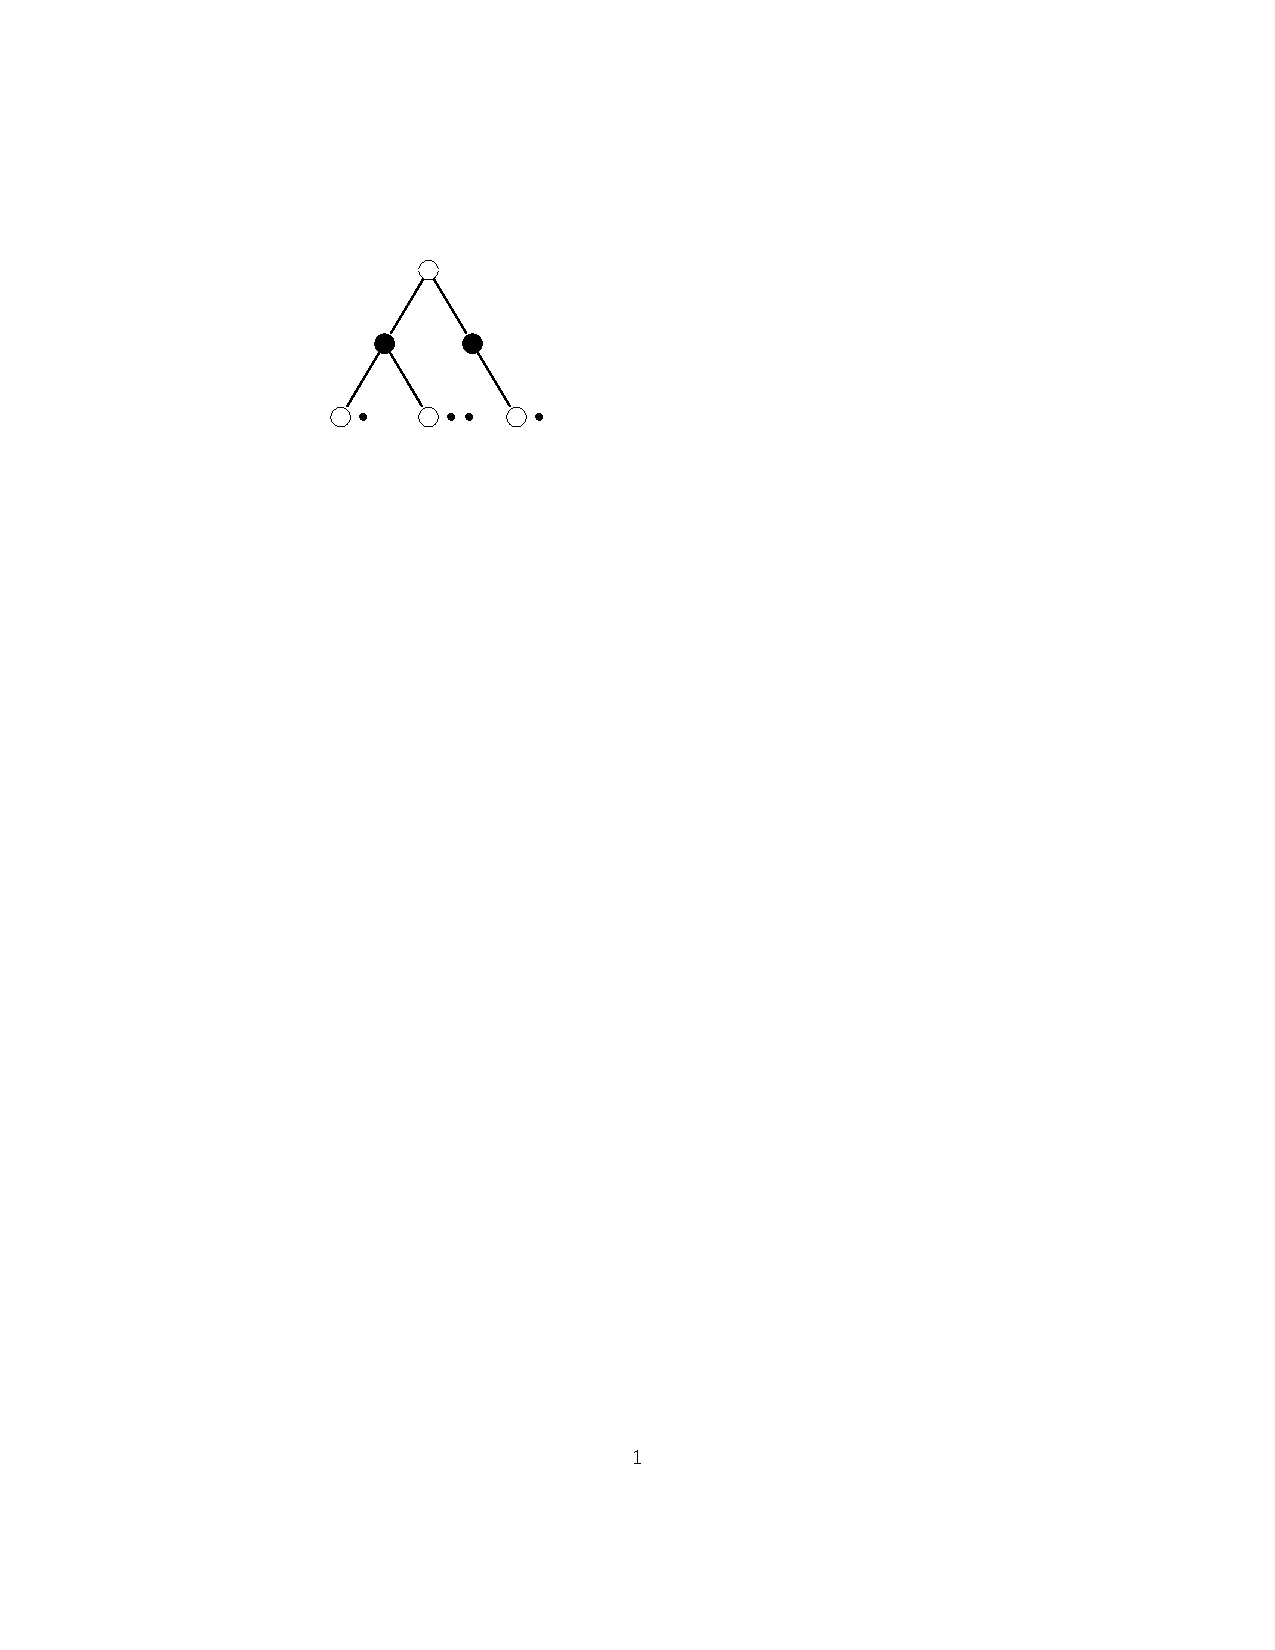
\includegraphics[width=0.7\linewidth, trim={5cm 17cm 12cm 4cm},clip]{articles/smcp/figures/main_ts1.pdf}
  \caption{\textbf{Configuration at time $t-1$:} we have the root white node $s_{t-1}$, the actions $a^{(n)}_{t-1}$ are black nodes and the leaf nodes are the $s^{(n)}_t$. We have one particle on the leftmost branch, two on the central branch and one on the rightmost branch. }
  \label{fig:sub1}
\end{subfigure}\hspace{.03\linewidth}
\begin{subfigure}{.30\textwidth}
  \centering
  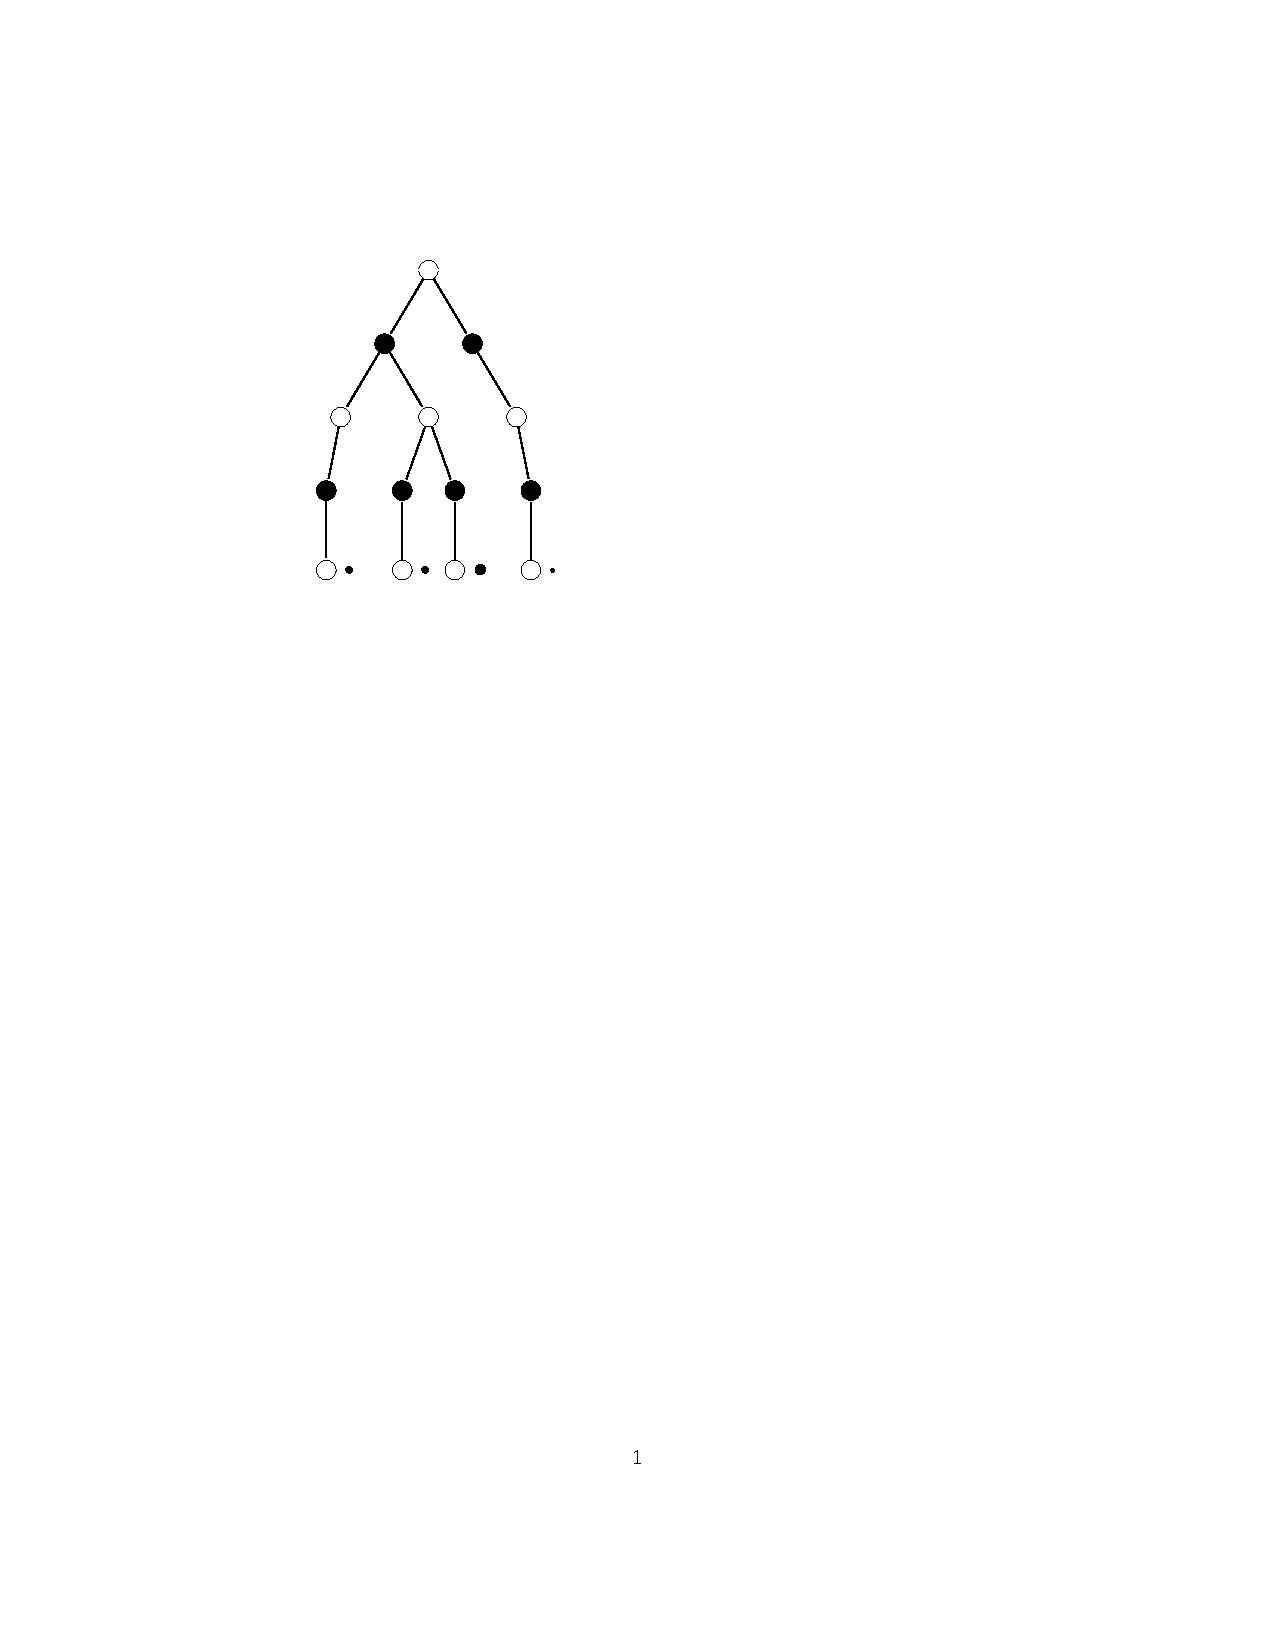
\includegraphics[width=0.7\linewidth, trim={5cm 17cm 12cm 4cm},clip]{articles/smcp/figures/main_ts4.pdf}
  \caption{\textbf{Update:} New actions and states are sampled from the proposal distribution and model. The particle sizes are proportional to their importance weight $w_t$.  \vspace{3.5em} } %
  \label{fig:sub2}
\end{subfigure}\hspace{.03\linewidth}
\begin{subfigure}{.30\textwidth}
  \centering
  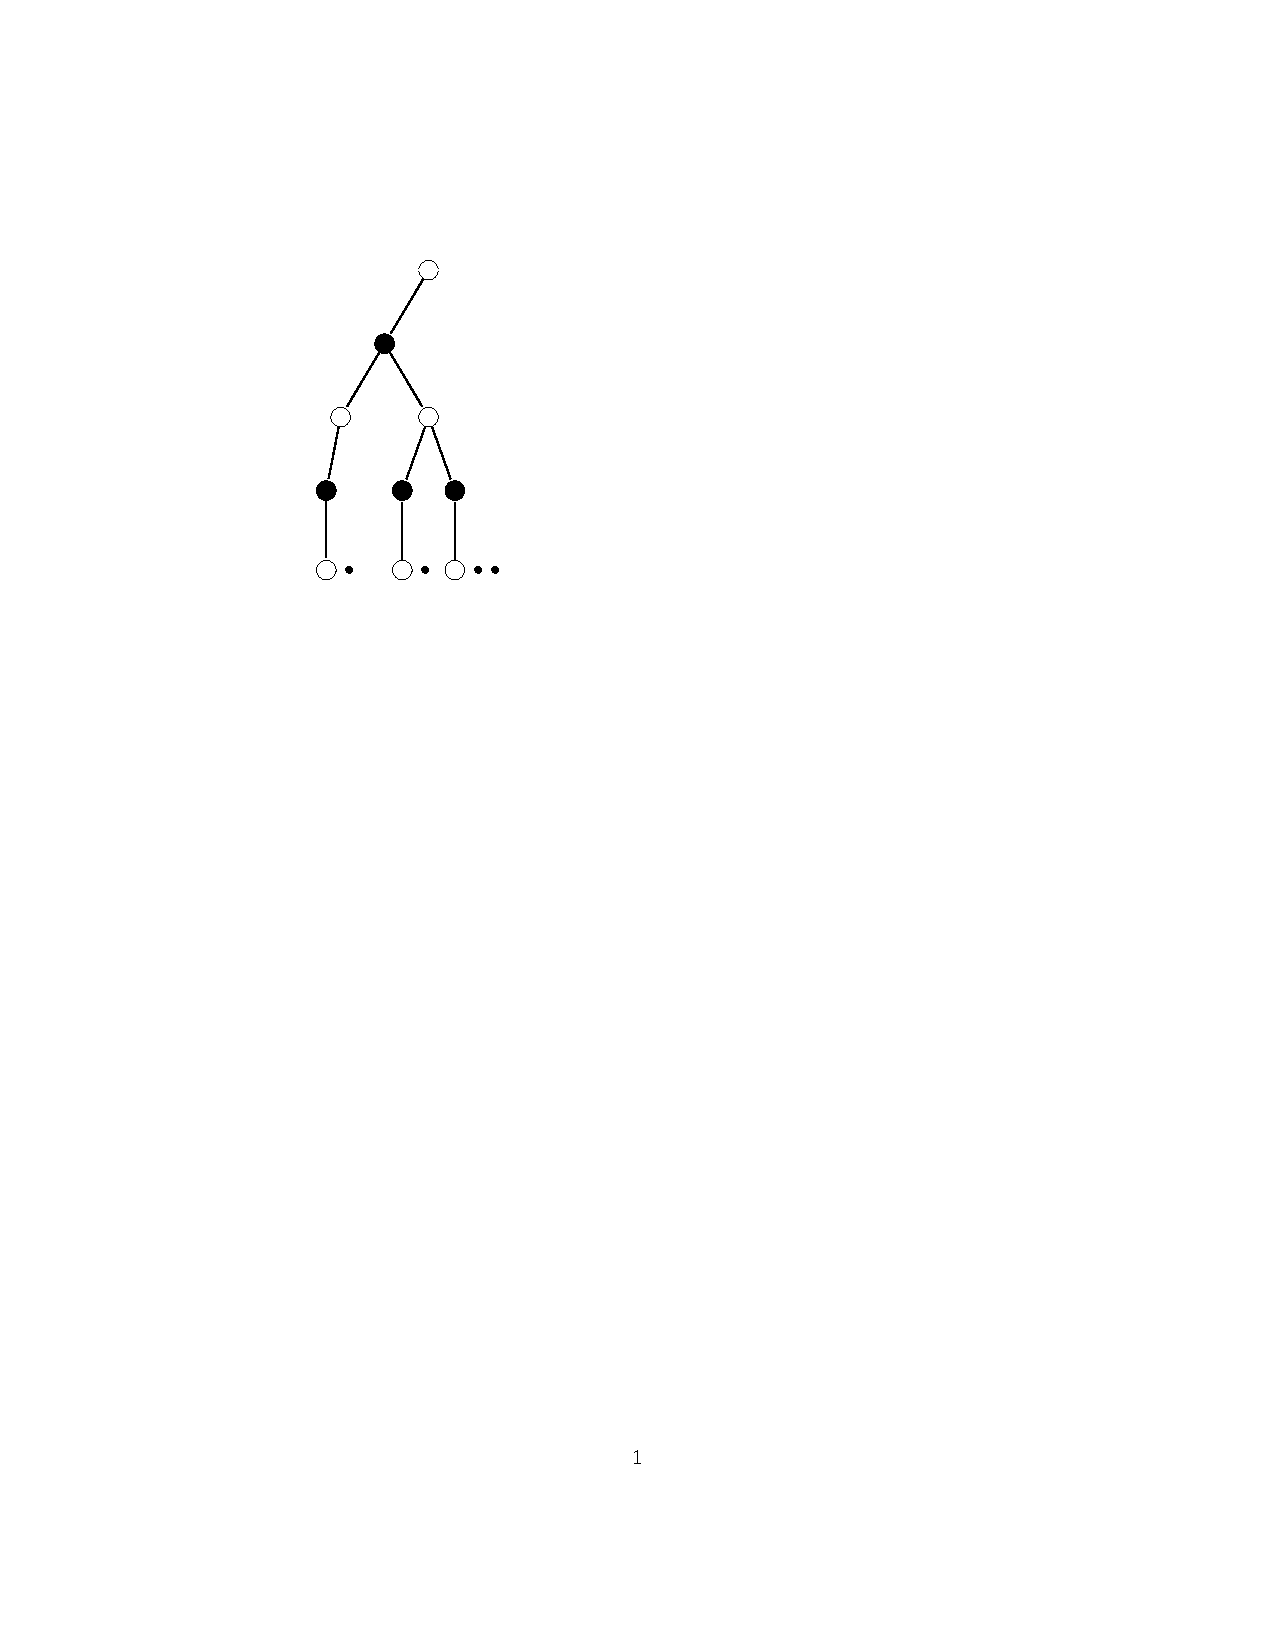
\includegraphics[width=0.7\linewidth, trim={5cm 17cm 12cm 4cm},clip]{articles/smcp/figures/main_ts5.pdf}
  \caption{\textbf{Resampling:} after sampling with replacement the particles relatively to their weight, the less promising branch was cut while the most promising has now two particles.\vspace{3em}}
  \label{fig:sub3}
\end{subfigure}
\caption{Schematic view of Sequential Monte Carlo planning. In each tree, the white nodes represent states and black nodes represent actions. Each bullet point near a state represents a particle, meaning that this particle contains the total trajectory of the branch. The root of the tree represents the root planning state, we expand the tree downward when planning.}
\label{fig:tree}
\end{figure}

\subsection{Optimism Bias and Control as Inference}
We now discuss shortcomings our approach to planning as inference may suffer from, namely encouraging risk seeking policies.

\paragraph*{Bias in the objective:} Trajectories having a high likelihood under the posterior defined in Equation~\ref{eq:posterior_target} are not necessarily trajectories yielding a high \textit{mean} return. Indeed, as 
$\log \E_p  \big[\exp R(\traj) \big] \ge  \E_p  \big[ R(\traj) \big]$
we can see that the objective function we maximize is an \textit{upper bound} on the quantity of interest: the mean return.
This can lead to risk-seeking trajectories as one very good outcome in $\log \E \exp$ could dominate all the other potentially very low outcomes, even if they might happen more frequently. This fact is alleviated when the dynamics of the environment are close to deterministic~\citep{levine2018reinforcement}. Thus, this bias does not appear to be very detrimental to us in our experiments~\ref{sec:exp} as our environments are fairly close to deterministic. The bias in the objective also appears in many control as inference works such as Particle Value Functions~\citep{maddison2017particle} and the probabilistic version of LQR proposed in~\cite{toussaint2009robot}.

\paragraph*{Bias in the model:} A distinct but closely related problem arises when one trains jointly the policy $\pi_\parampol$ and the model $\pmodel$, i.e if $q(\traj_{1:T})$ is directly trained to approximate $p(\traj_{1:T} | \gO_{1:T})$. In that case, $\pmodel(s_{t+1} | s_t, a_t)$ will not approximate $\penv(s_{t+1} | s_t, a_t)$ but $\penv(s_{t+1} | s_t, a_t, \gO_{t:T})$~\citep{levine2018reinforcement}. This means the model we learn has an optimism bias and learns transitions that are overly optimistic and do no match the environment's behavior.
This issue is simply solved by training the model separately from the policy, on transition data contained in a buffer as seen on line 18 of Algorithm~\ref{alg:sir_planning}.


\section{Experiments}
\subsection{Toy example}

In this section, we show how SMCP can deal with multimodal policies when planning.
We believe multimodality is useful for exploring since it allows us to keep a distribution over many promising trajectories and also allows us to adapt to changes in the environment e.g. if a path is suddenly blocked.

We applied two version of SMCP: i) with a resampling step (SIR) ii) without a resampling step (SIS) and compare it to CEM on a simple 2D point mass environment~\ref{fig:toy}. Here, the agent can control the displacement on $(x,y)$ within the square $[0,1]^2$, $a = (\Delta x, \Delta y)$ with maximum magnitude $||a|| = 0.05$. The starting position ($\bullet$) of the agent is $(x=0, y=0.5)$, while the goal ({\color{red} $\star$}) is at $g = (x=1, y=0.5)$. The reward is the agent's relative closeness increment to the goal: $r_t = 1- \frac{||s_{t+1} -g||^2}{||s_t -g||^2}$. However, there is a partial wall at the centre of the square leading to two optimal trajectories, one choosing the path below the wall and one choosing the path above.

The proposal is an isotropic normal distribution for each planning algorithm, and since the environment's dynamics are known, there is no need for learning: the only difference between the three methods is how they handle planning. We also set the value function to $0$ for SIR and SIS as we do not wish to perform any learning. We used $1500$ particles for each method, and updated the parameters of CEM until convergence. Our experiment~\ref{fig:toy} shows how having particles can deal with multimodality and how the resampling step can help to focus on the most promising trajectories. 



\begin{figure}
\begin{subfigure}{.295\textwidth}
\centering
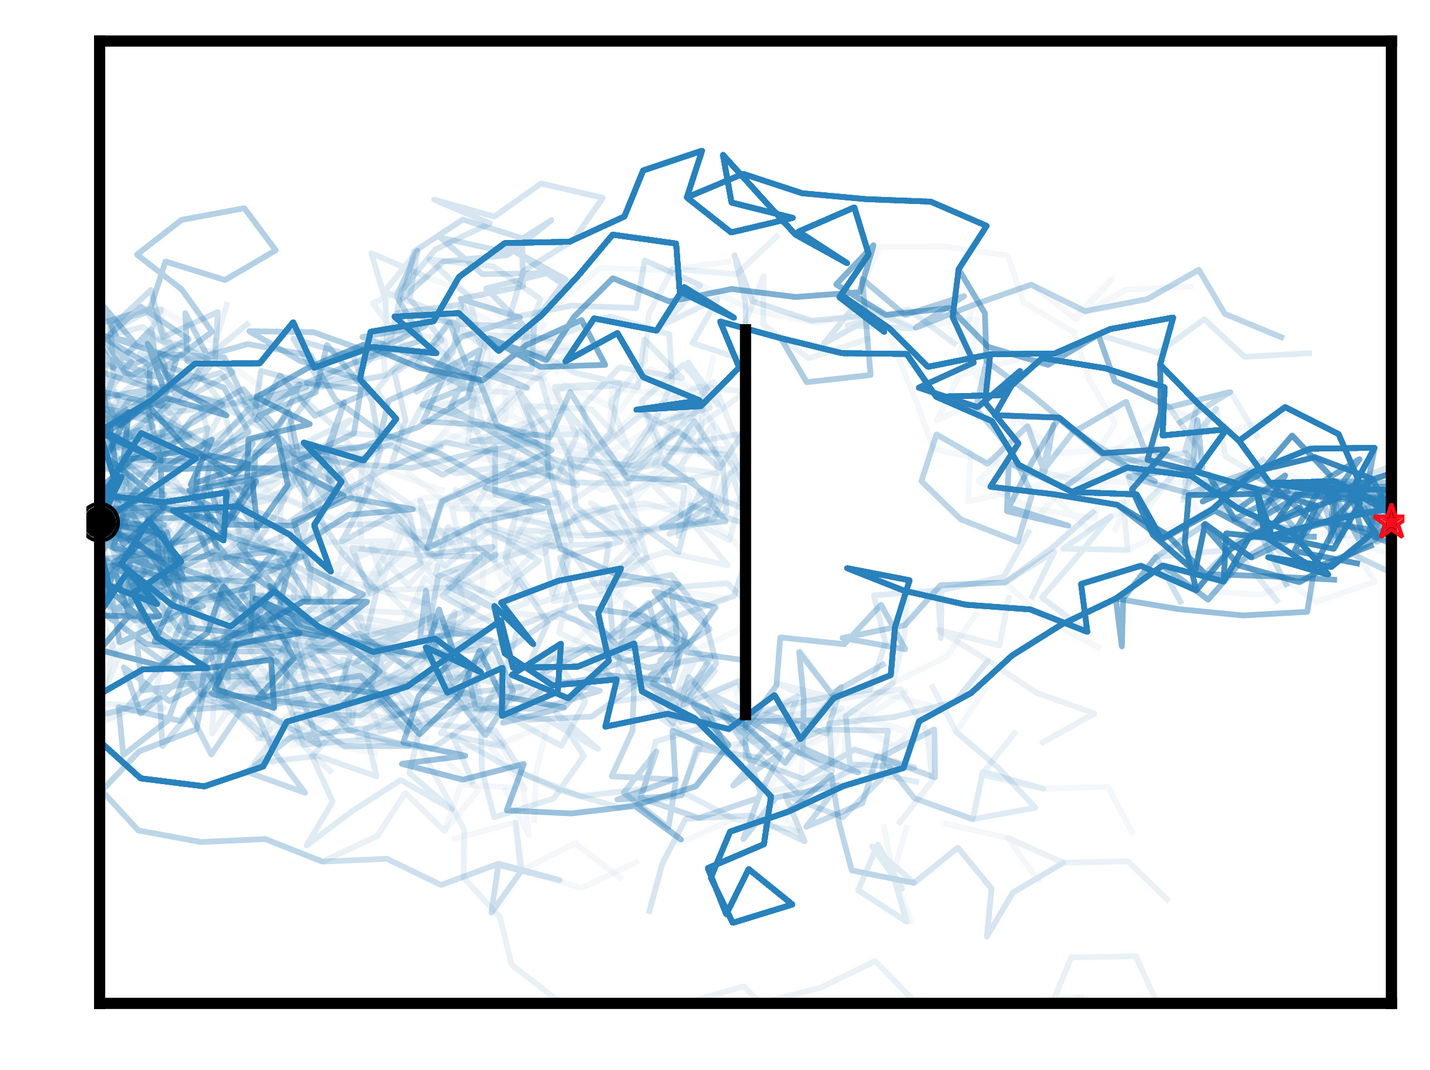
\includegraphics[width=\linewidth, trim={1.1cm 0cm .5cm 0cm},clip]{articles/smcp/figures/smc_resampling_true.png}
\caption{Sequential Importance Resampling (SIR): when resampling the trajectories at each time step, the agent is able to focus on the promising trajectories and does not collapse on a single mode.}
\label{fig:toy_sir}
\end{subfigure}\hspace{0.05\linewidth}
\begin{subfigure}{.295\textwidth}
\centering
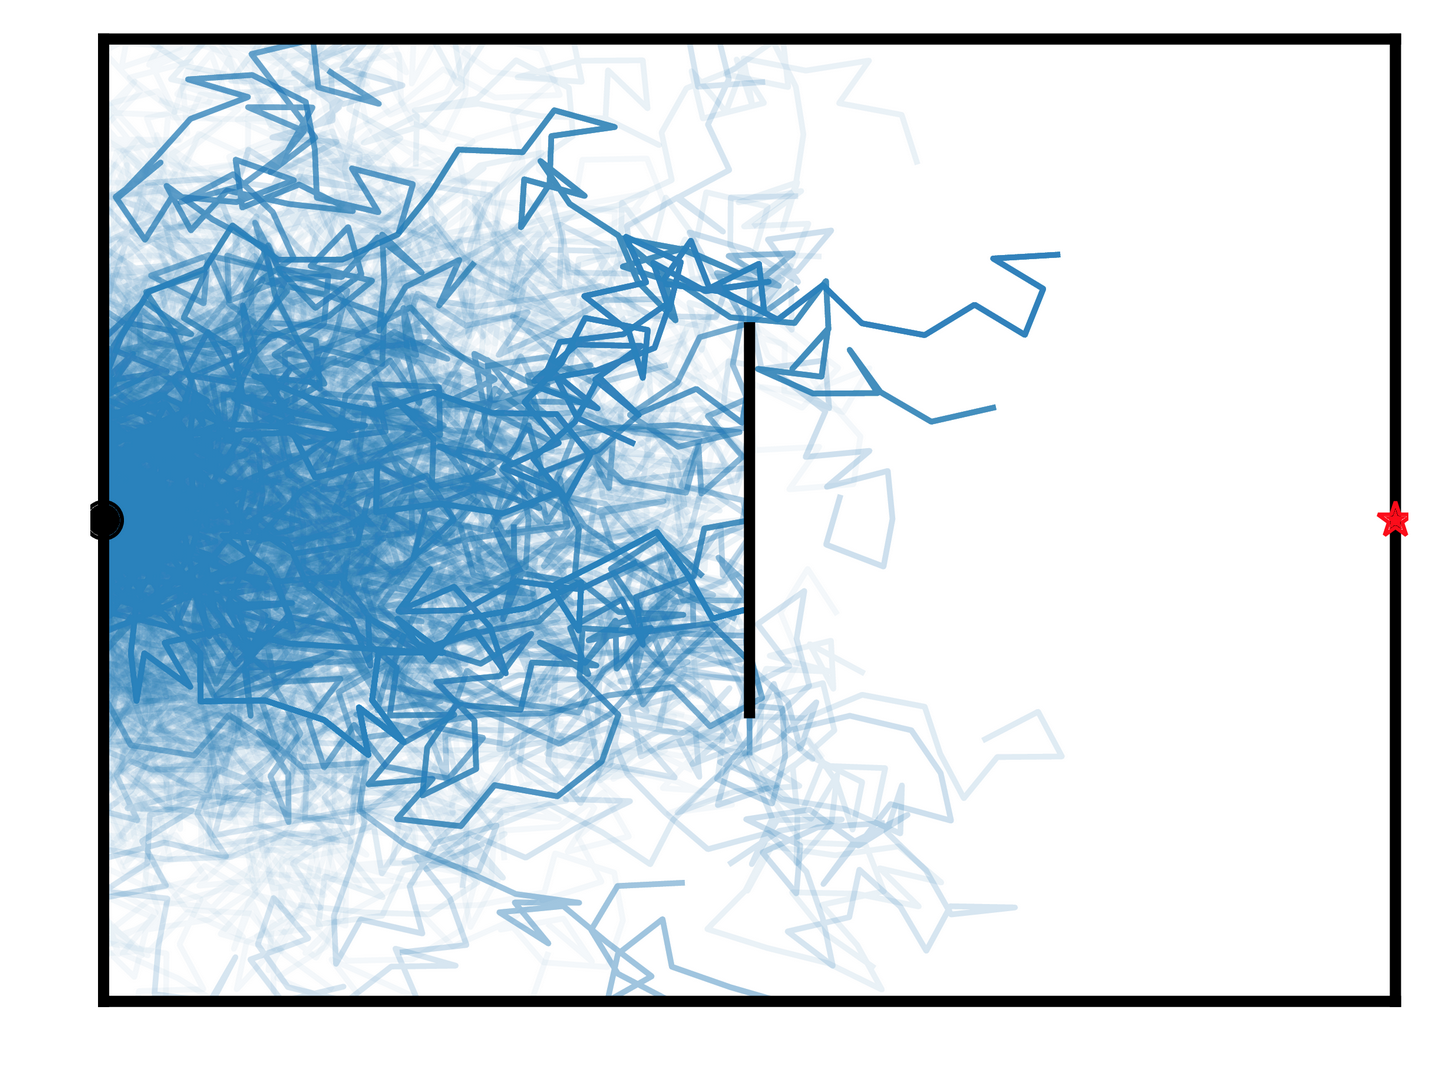
\includegraphics[width=\linewidth, trim={1.1cm 0cm .5cm 0cm},clip]{articles/smcp/figures/smc_resampling_false.png}
\caption{Sequential Importance Sampling (SIS): if we do not perform the resampling step the agent spends most of its computation on uninteresting trajectories and was not able to explore as well.\vspace{1em}}
\label{fig:toy_sis}
\end{subfigure}\hspace{0.05\linewidth}
\begin{subfigure}{.295\textwidth}
\centering
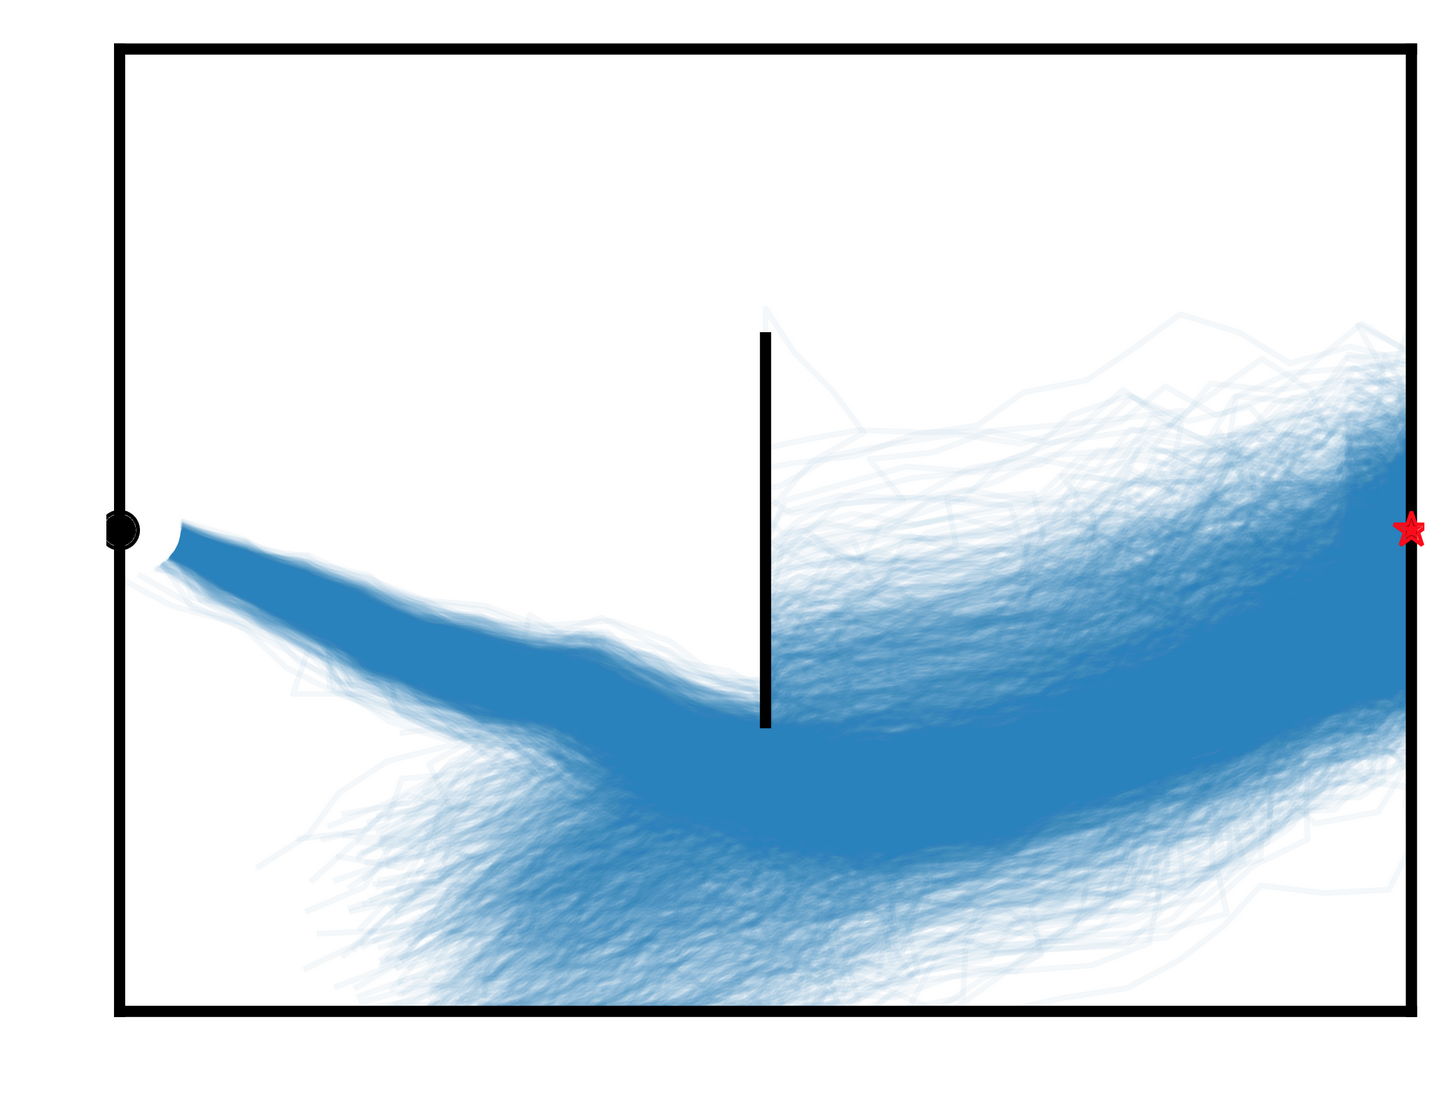
\includegraphics[width=\linewidth, trim={1.1cm 0cm .5cm 0cm},clip]{articles/smcp/figures/cem.png}
\caption{CEM: here the agent samples all the actions at once from a Gaussian with learned mean and covariance. We needed to update the parameters 50 times for the agent to find one solution, but it forgot the other one. }
\label{fig:toy_cem}
\end{subfigure}
\caption{Comparison of three methods on the toy environment. The agent ($\bullet$) must go to the goal ({\color{red}$\star$}) while avoiding the wall (\ \textbf{\textbar}\ ) in the center. The proposal distribution is taken to be an isotropic gaussian.  Here we plot the planning distribution imagined at $t=0$ for three different agents.  A darker shade of blue indicates a higher likelihood of the trajectory. Only the agent using Sequential Importance Resampling was able to find good trajectories while not collapsing on a single mode.}
\label{fig:toy}
\end{figure}

\subsection{Continuous Control Benchmark}
\label{sec:exp}

The experiments were conducted on the Open AI Gym Mujoco benchmark suite \citep{brockman2016openai, todorov2012mujoco}. To understand how planning can increase the learning speed of RL agents we focus on the 250000 first time steps. The Mujoco environments provide a complex benchmark with continuous states and actions that requires exploration in order to achieve state-of-the-art performances. 

The environment model used for our planning algorithm is the same as the probabilistic neural network used by \citet{chua2018deep}, it minimizes a gaussian negative log-likelihood model: 
\begin{equation*}
    \mathcal{L}_{\text{Gauss}}(\theta)= \tfrac{1}{2}\sum_{n=1}^N[\mu_\theta(s_n, a_n)-(s_{n+1}-s_n)]^\top\Sigma^{-1}_\theta(s_n, a_n)[\mu_\theta(s_n, a_n)-(s_{n+1}-s_n)]+\log \text{det} \Sigma_\theta(s_n, a_n),
\end{equation*}

where $\Sigma_\theta$ is diagonal and the transitions $(s_n, a_n, s_{n+1})$ are obtained from the environment.%





We included two popular planning algorithms on Mujoco as baselines: CEM \citep{chua2018deep} and Random Shooting (RS) \citep{nagabandi2017neural}. Furthermore, we included SAC \citep{haarnoja2018soft}, a model free RL algorithm, since i) it has currently one of the highest performances on Mujoco tasks, which make it a very strong baseline, and ii) it is a component of our algorithm, as we use it as a proposal distribution in the planning phase.

Our results suggest that SMCP does not learn as fast as CEM and RS initially as it heavily relies on estimating a good value function. However, SMCP quickly achieves higher performances than CEM and RS. SMCP also learns faster than SAC because it was able to leverage information from the model early in training. We hypothesize that the lack of performance gain of SMCP over SAC in the Hopper environment is due to the low quality of its model and the complexity of the task.

Note that our results differ slightly from the results usually found in the model-based RL literature. This is because we are tackling a more difficult problem: estimating the transitions and the reward function. We are using unmodified versions of the environments which introduces many hurdles. For instance, the reward function is challenging to learn from the state and very noisy. %

As in~\citet{henderson2017deep}, we assess the significance of our results by running each algorithm with multiple seeds ($10$ random seeds in our case, from seed $0$ to seed $9$). %






\begin{figure}
\centering
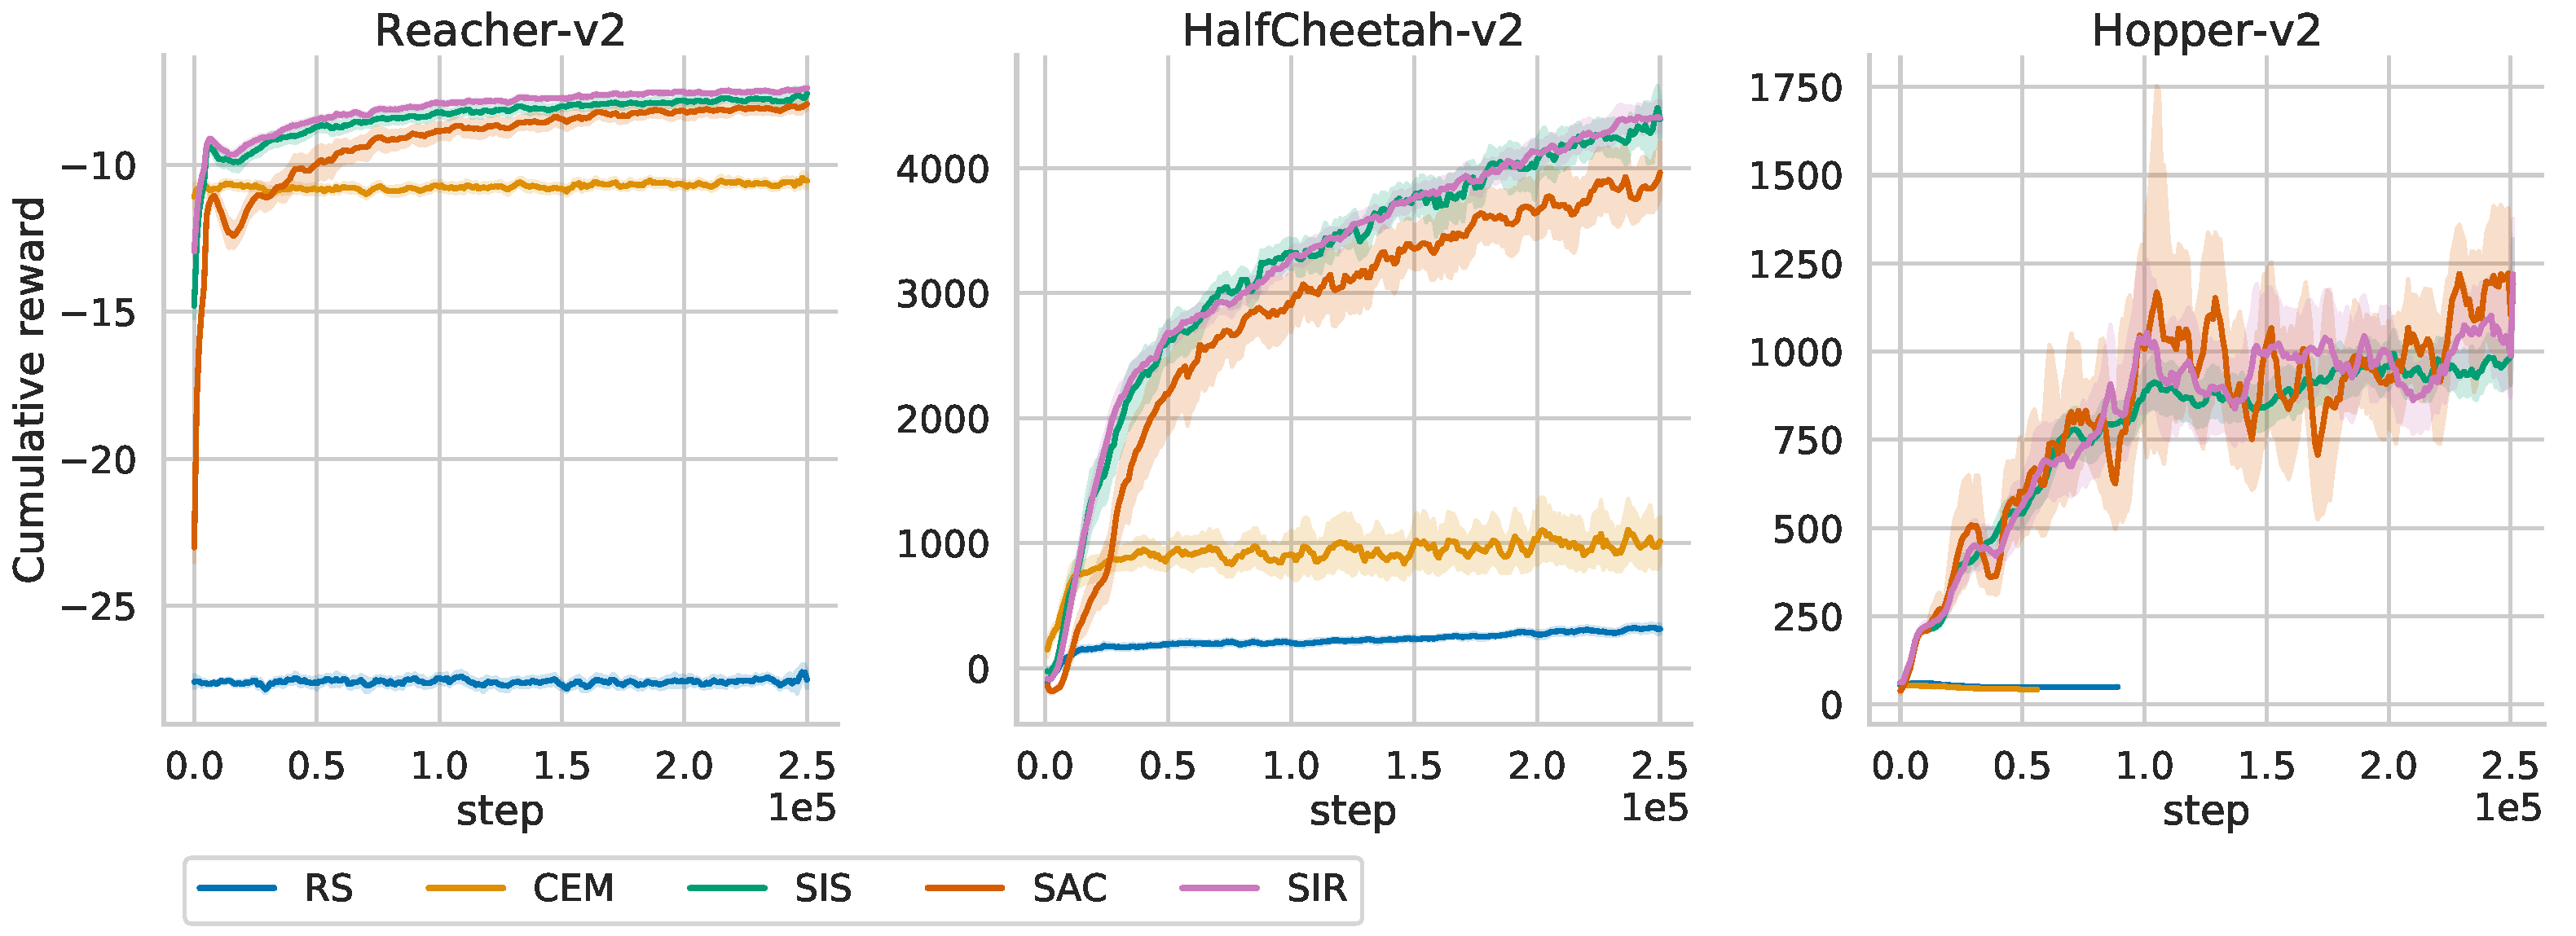
\includegraphics[width=\linewidth]{articles/smcp/figures/finalplotsmcp.pdf}
\caption{
Training curves on the Mujoco continuous control benchmarks. Sequential Monte Carlo Planning both with resampling (SIR) (pink) and without (SIS) (orange) learns faster than the Soft Actor-Critic model-free baseline (blue) and achieves higher asymptotic performances than the planning methods (Cross Entropy Methods and Random Shooting). The shaded area represents the standard deviation estimated by bootstrap over 10 seeds as implemented by the Seaborn package.  %
}
\label{fig:reward_new}
\end{figure}









\section{Conclusion and Future Work}
In this work, we have introduced a connection between planning and inference and showed how we can exploit advances in deep learning and probabilistic inference to design a new efficient and theoretically grounded planning algorithm. 
We additionally proposed a natural way to combine model-free and model-based reinforcement learning for planning based on the SMC perspective.
We empirically demonstrated that our method achieves state of the art results on Mujoco. Our result suggest that planning can lead to faster learning in control tasks.

However, our particle-based inference method suffers some several shortcomings. First, we need many particles to build a good approximation of the posterior, and this can be computationally expensive since it requires to perform a forward pass of the policy, the value function and the model for every particle. Second, resampling can also have adverse effects, for instance all the particles could be resampled on the most likely particle, leading to a particle degeneracy. More advanced SMC methods dealing with this issue such as backward simulation~\citep{lindsten2013backward} or Particle Gibbs with Ancestor Sampling (PGAS)~\citep{lindsten2014particle} have been proposed and using them would certainly improve our results.

Another issue we did not tackle in our work is the use of models of the environment learned from data. Imperfect model are known to result in compounding errors for prediction over long sequences. We chose to re-plan at each time step (Model Predictive Control) as it is often done in control to be more robust to model errors. More powerful models or uncertainty modeling techniques can also be used to improve the accuracy of our planning algorithm.
While the inference and modeling techniques used here could be improved in multiple ways, SMCP achieved impressive learning speed on complex control tasks. The planning as inference framework proposed in this work is general and could serve as a stepping stone for further work combining probabilistic inference and deep reinforcement learning.


